\section{Our Proposed Method}

%overview
In this section, we describe our system for sentiment classification in a lifelong learning setting, which is a combination of components to analyze reviews from many domains.
The system takes customer reviews, from multiple types of products, as source domains.
Each review can contain multiple sentences and it is labeled positive, negative or neutral based on how users rated them.
From the source domains mentioned above, the system gains knowledge valuable to the learning task on the target domain.
Such knowledge is used to optimize the classifier on the target domain using stochastic gradient descent (SGD).
          
%như title
\subsection{Overview of lifelong learning for sentiment classification}
As described in figure~\ref{figure: LLL}, the system contains three main modules: knowledge storing, optimization, and sentiment classification.

\begin{figure}
	\centering                                    
	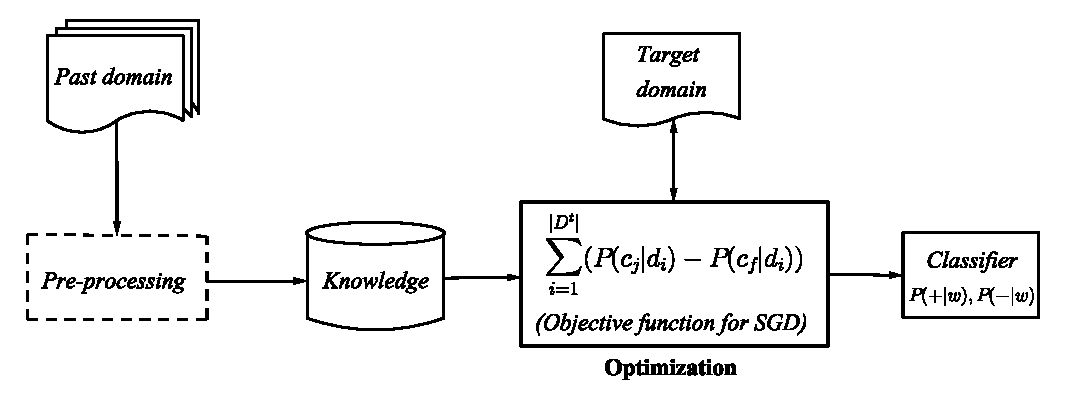
\includegraphics[height=4.35cm]{process_vector}
	\caption{Lifelong learning for sentiment classification}
	\label{figure: LLL}
\end{figure}

\subsubsection{Knowledge storing}
The system extracts knowledge from the past domains, which is used to optimize the classifier on the target domain.
There are three types of knowledge, including:
%do the reviewers have to know these?
\begin{itemize}
	\item
	The Prior probability $P^t_+(w|c)$ and $P^t_-(w|c)$ of each word, where t is a past learning task.
	%Because we choose to combine Naïve Bayes and bigram feature, $
	\item
	Number of times a word appears in positive or negative in learning task: $N^t_{+,w}$, $N^t_{-,w}$.
	Similarly, the number of occurrences of $w$ in the positive and negative documents are respectively $N^{KB}_{+,w}= \sum{N^t_+}$ and $N^{KB}_{-,w} = \sum{N^t_-}$
	\item
	Number of past tasks in which $P_{w|+}>P_{w|-}$ or vice versa: $M^{KB}_{+,w}$, $M^{KB}_{-,w}$.
	The two figures are used to leverage domain knowledge via a penalty term to penalize the words that appear in just a few domains. %less than a reasonable number of domains
\end{itemize}

\subsubsection{Optimization}
With the help of all three types of knowledge mentioned above, this component is used to optimize the objective function on the training set of the target domain. %to get the most optimized classifier for testing.
The objective function is $\sum_{i=1}^{|D_i|}{P(c_j|d_i)-P(c_f|d_i)} $ , in which $c_j$ is the actual labeled class, $c_f$ is the wrong class of the document $d_i$.
We follow the SGD with similar regularization techniques proposed by Chen et al.~\cite{chen-ma-liu:2015:ACL-IJCNLP}.
Our optimized variables are $X_{+,w}$ and $X_{-,w}$, which are the occurrences of a word $w$ in a positive and negative class, respectively. 
The objective function is optimized on each document of the target domain until convergence.
After SGD, we use Bayes formula (see equation~\ref{equa:nb+},~\ref{equa:nb-}) to create a classifier optimized for the target domain. 
Note that Laplace smoothing is applied in both cases.
\begin{equation}
P(+|w)= \frac{\lambda + X_{+,w}}{\lambda|V|+\sum_{v=1}^{V}{X_{+,v}}}
\label{equa:nb+}
\end{equation}
\begin{equation}
P(-|w)= \frac{\lambda + X_{-,w}}{\lambda|V|+\sum_{v=1}^{V}{X_{-,v}}}
\label{equa:nb-}
\end{equation}

\subsubsection{Sentiment classification}
With the classifier optimized for the target domain, the system does sentiment classification task on each document of the test domain. 
Although the approach still follows Naïve Bayes framework, the way we classify differentiates between unigrams, bigrams, and bag-of-bigrams.



\subsection{Bigrams}
%bigram illustration
We propose the use of bigram feature, instead of unigram, on this type of sentiment classification.
Wang and Manning~\cite{wang-manning:2012:ACL2012short} has proved that using bigram always improve the performance on sentiment classification.
%Due to the fact that there are a lot of phrases that can express sentiment in the documents, the bigram feature can help improve the original Naive Bayes framework applying unigram feature with classifier 
For instance, phrases such as ``have to'' in English or ``không thích'' (dislike) in Vietnamese can express sentiment well in the documents.
These noun phrases and verb phrases cannot be captured by using unigram feature alone.
%Hence, using bigram feature captures modified and nouns.
%Bigram feature also helps capture (adjective + noun), (verb + adverb).e.g phrases in both Vietnamese and English.
%The modified model we choose to combine Naïve Bayes and bigram feature is described below:

The way we integrate bigram feature into Naïve Bayesian framework for lifelong learning is described below:

\begin{itemize}
	
\item In \textbf{Knowledge storing} step, beside $P^t_+(w|c)$ and $P^t_-(w|c)$, we also store $P^t_+(w_i|w_{i-1})$ and $P^t_-(w_i|w_{i-1})$ whereas $P^t_+(w_{i+1}|w_i) = \frac{\lambda + N_{+,w_iw_{i+1}}}{\lambda|V|+N_{+,w_i}}$ and $P^t_-(w_{i+1}|w_i)= \frac{\lambda + N_{-,w_iw_{i+1}}}{\lambda|V|+N_{-,w_i}}$). 
The number of occurrences of each bigram on each class ($N^t_{+,w_iw_{i+1}}$ and $N^t_{-,w_iw_{i+1}}$) and the domain-level knowledge  ($M^{KB}_{+,w_iw_{i+1}}$, and  $M^{KB}_{-,w_iw_{i+1}}$) are also stored. 
			
\item In \textbf{Optimization} step, due to the use of bigram, the probability for each document is modified as equations~\ref{pdoc+},~\ref{Pdoc-}:
\begin{equation}
P(+|d) = \frac{P_+}{P_-}.P_+(w_0).P_+(w_1|w_0).P_+(w_2|w_1)…P_+(w_n|w_{n-1}) 
\label{pdoc+}
\end{equation}

\begin{equation}
P(-|d) = \frac{P_-}{P_+}.P_-(w_0).P_-(w_1|w_0).P_-(w_2|w_1)…P_-(w_n|w_{n-1}) 
\label{Pdoc-}
\end{equation}

\item The positive and negative probabilities for each document on the test data also have to follow the equations~\ref{pdoc+},~\ref{Pdoc-} for the \textbf{Sentiment Classification} step.

\end{itemize}

\subsection{Bag of bigrams} %better performance, relies on probability of unigram
%bag-of-bigrams illustration
Although using bigram help taking advantage of the phrases that express sentiments, using the standard Bayes formula still relies on the probabilities and number of occurrences of unigrams on all the documents.
Our alternative way to leverage bigram is to treat each bigram as a unigram and apply the normally used Bayes formula ( $P_{+|d} = \frac{P_+}{P_-}.P_+(w_0w_1).P_+(w_1w_2).P_+(w_2w_3)…P_+(w_{n-1}w_n) $) to create the classifier.
Such formula is applied to \textbf{Optimization} and \textbf{Sentiment classification} steps. 
%This bag-of-bigram approach help reduce the size of vocabulary set to contains only bigrams instead of both, which decrease the required time to complete the task.
%In experimental results, we will compare how the two solutions improve the classification performance on both Vietnamese and English dataset.
We will compare how the two solutions improve the classification performance on both Vietnamese and English dataset.

\subsection{Pre-Processing on Vietnamese dataset}
Different to the dataset from Chen et al.~\cite{chen-ma-liu:2015:ACL-IJCNLP} on English, the Tiki.vn dataset contains many emoticons. 
Therefore, we need to pre-process the data before \textbf{Knowledge storing} step to leverage all lexical resources in the dataset. 
In most online forums or discussion groups, users often use emoticons such as ``:)'', ``:('' or punctuations such as ``!!!!!'' to express their opinions.
However, during the task, we standardize the emoticons used by users, e.g. changing ``:((((('' to ``:(''.
We treat each emoticon or punctuation as a unigram and follow the other steps as normal.
%This approach has slightly improved our performance on Vietnamese dataset.
In this pre-processing step, we also perform word segmentation by following the maximum entropy approach of Dinh and Vu~\cite{DDien-VThuy:2006}.
Word segmentation can model the sentiment adjectives which often contain two or more morphemes, hence, provide a better vocabulary set for classification on Vietnamese using unigram feature.

%\item \textbf{Optimization}: This component follow the stochastic gradient descent with similar regularization techniques proposed by Chen et al.~\cite{chen-ma-liu:2015:ACL-IJCNLP}.
%The component will use the knowledge above to update the virtual count $X$ until convergence to get the best classifier for the target domain.
%\item \textbf{Sentiment classification}: With the classifier optimized for the target domain, the system does sentiment classification task on each document of the test domain %To have a truly overall view of lifelong learning for Vietnamese sentiment classification, we test the classifier which is just optimized for the target domain on different cases including segmentation and without segmentation task, unigram feature and bigram feature, with and without stop words.

%This component is to process the reviews, especially the raw reviews of the Vietnamese dataset, in a suitable type.
%%On our dataset, the average unigram per document on each domain varies from 66 to just above 75 unigrams.
%The input collection includes a number of past domains and one target domain.
%The knowledge gained from the input domain will be used to add values to the learning task on the target domain.
%%Finally, with refined parameters, the system will classify reviews on the testing part of the target domain.
%
%The system contains three main modules: storing knowledge, optimization, and sentiment classification.
%
%% Storing knowledge
%
%% optimization
%
%% sentiment classification
%

%
%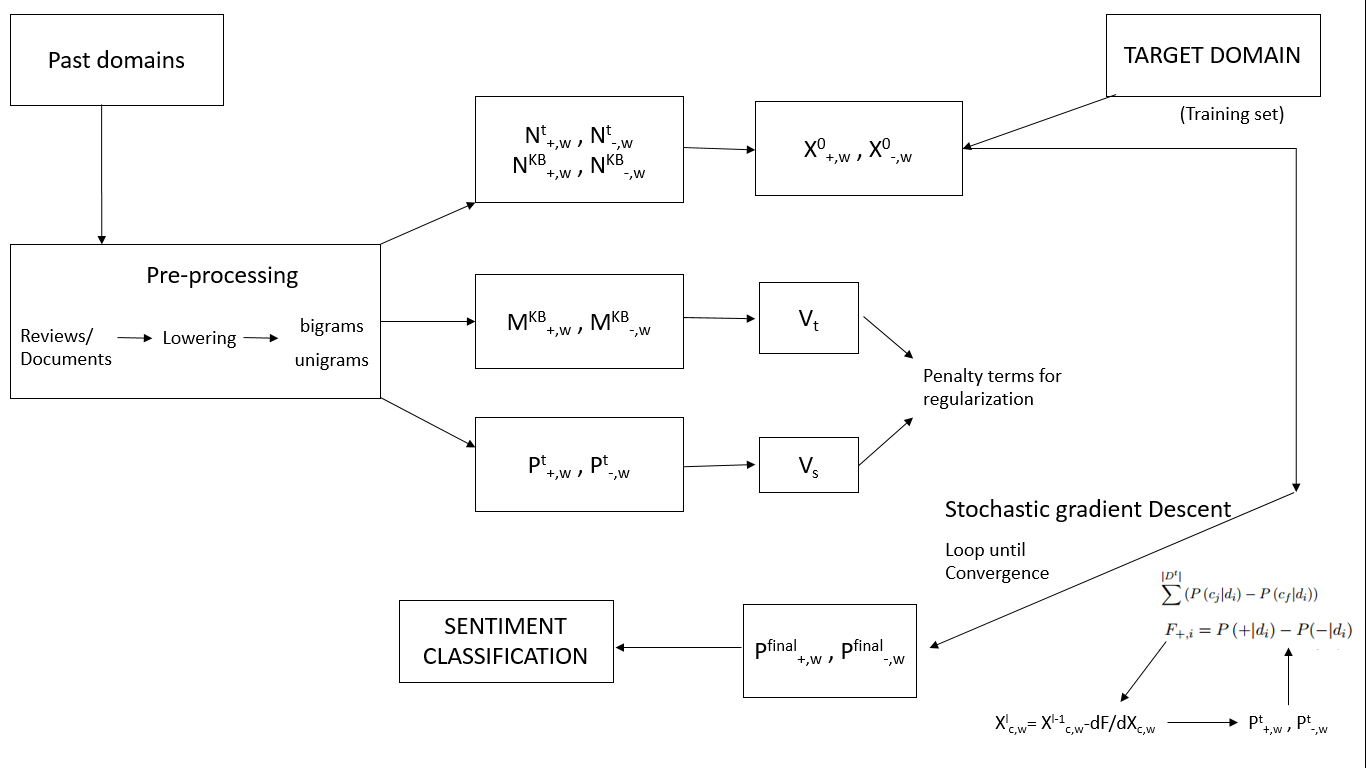
\includegraphics[scale=0.2]{system}
%
%\begin{itemize}
%	\item \textbf{Storing knowledge}: This component is to process the reviews from the past domains and gain the parameters for learning task on the target domain.
%	Since Vietnamese is an isolated language, we follow the maximum entropy approach of Dinh and Vu~\cite{DDien-VThuy:2006} to segment each document on the Vietnamese dataset.
%	The segmentation task can help better modeling the sentiment adjectives which often contains two or more syllables, hence, provide a better vocabulary set for classification on Vietnamese using unigram feature.
%	On both English and Vietnamese dataset, each review is tokenized into unigrams and bigrams to help us experiment both cases.
%	After the text processing tasks, the system will try to extract the knowledge that will be used to optimize the classifier on the target domain.
%	The main types of knowledge consists of: